\chapter{Data Preprocessing}
\label{chap:data_preprocessing}

In this chapter, we perform essential preprocessing steps to ensure the datasets are clean, balanced, and suitable for training robust models. Each preprocessing step is carefully designed to address specific challenges commonly encountered in real-world datasets.

\section{Fashionopedia Dataset}

\subsection{Removing Invalid Bounding Boxes}

The dataset initially contains bounding box annotations for various objects within images. However, some of these bounding boxes are invalid — they have zero width or height (i.e., $x_{\text{min}} = x_{\text{max}}$ or $y_{\text{min}} = y_{\text{max}}$). In this step, all invalid bounding boxes are systematically detected and removed. For each image, only bounding boxes with positive area are retained, along with their associated IDs, categories, and area values. This ensures that the annotations are meaningful and correspond to real object regions.

\textbf{Significance:} Invalid bounding boxes can severely impact model training by introducing noise or errors, as object detection models rely heavily on accurate spatial localization. Cleaning the dataset at this stage helps maintain data quality, improves model stability, and ensures better learning dynamics.

After this step, the train and validation datasets maintain the same number of images (45,623 and 1,158 respectively), but contain only valid bounding boxes within each image.

\subsection{Visualizing Class Occurrences}

To gain insights into the dataset distribution, the number of occurrences for each object category was calculated and visualized. Each bounding box was mapped to its corresponding label, and a bar plot was generated to display the frequency of each category.

\begin{figure}[H]
\centering
    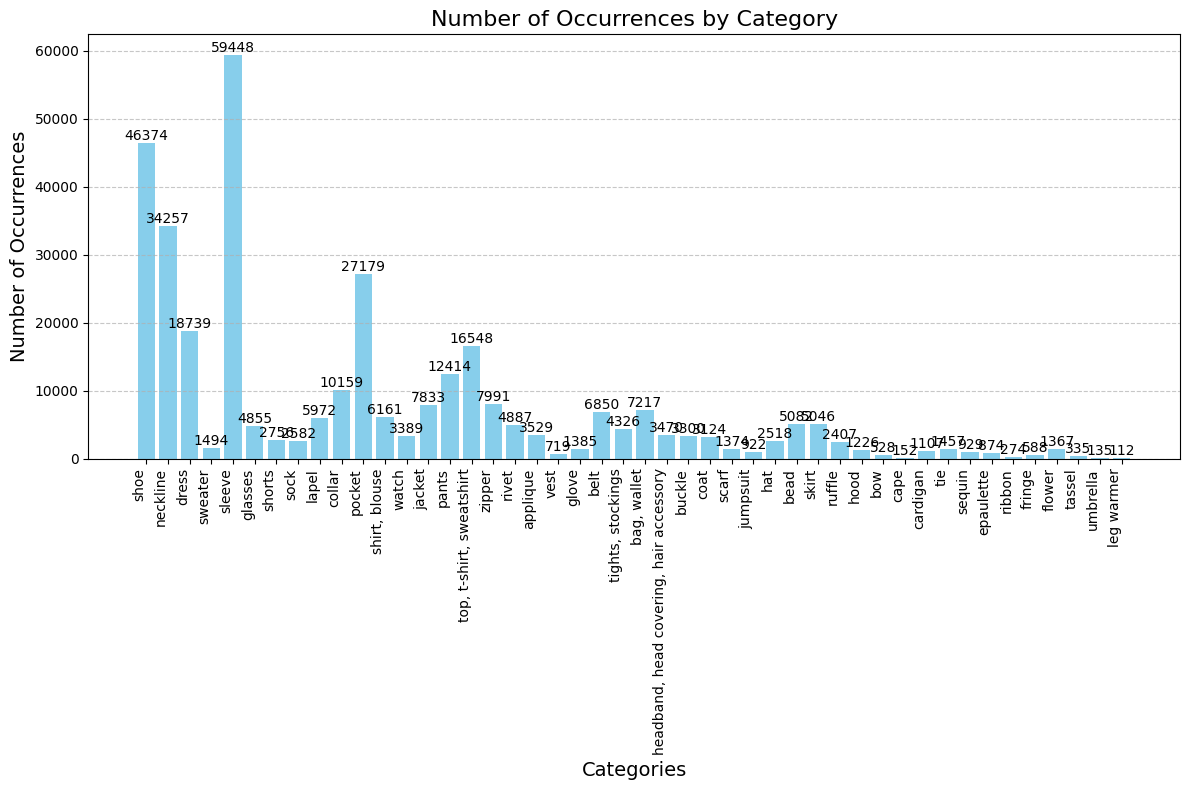
\includegraphics[width=0.8\textwidth]{images/classes.png}
\end{figure}

\textbf{Significance:} This analysis revealed that certain classes, such as ``shoe'' and ``sleeve'', are significantly overrepresented. Identifying such class imbalances early is critical, as models trained on imbalanced datasets are prone to biased predictions. Appropriate strategies, such as data augmentation, can be designed later to address this imbalance.

\subsection{Data Augmentation}

Data augmentation was performed to artificially increase dataset diversity and improve model generalization. Using the Albumentations library, the following transformations were applied:

\vspace{-1.25em}
\begin{itemize}
    \setlength\itemsep{-1.05em}
    \item \textbf{LongestMaxSize and PadIfNeeded:} Resize and pad images to a fixed size of $500 \times 500$ pixels, ensuring consistency in input dimensions.
    \item \textbf{Horizontal Flip:} Randomly flip images horizontally with a probability of 0.5 to introduce left-right invariance.
    \item \textbf{RandomBrightnessContrast and HueSaturationValue:} Apply color jittering to simulate different lighting conditions.
    \item \textbf{Rotation and Random Scale:} Introduce small random rotations and scale variations to improve spatial robustness.
    \item \textbf{Gaussian Blur and Gauss Noise:} Add blur and noise to simulate variations in image quality.
\end{itemize}

\begin{figure}[H]
\centering
    \includegraphics[width=0.8\textwidth]{images/augmented.png}
    \caption{Example of data augmentation applied to training images}
\end{figure}

For the validation set, only resizing and padding were applied to maintain a standardized evaluation environment without artificial noise.

\textbf{Significance:} Data augmentation is vital in object detection tasks where obtaining large, diverse datasets is often difficult. Augmentation helps prevent overfitting by exposing the model to a wider variety of object appearances, poses, and lighting conditions, ultimately leading to more robust performance on unseen data.

\subsection{Feature Extraction}

Images in the Fashionopedia dataset are stored as PIL Images. To prepare them for model training, they need to be transformed into numerical tensors. This was achieved using the YOLOS Feature Extractor.

The YOLOS feature extractor, pre-trained on a variety of datasets, standardizes images by resizing them and applying necessary transformations such as normalization. The feature extractor converts each image into a set of values that are better suited for model ingestion.

\begin{figure}[H]
\centering
    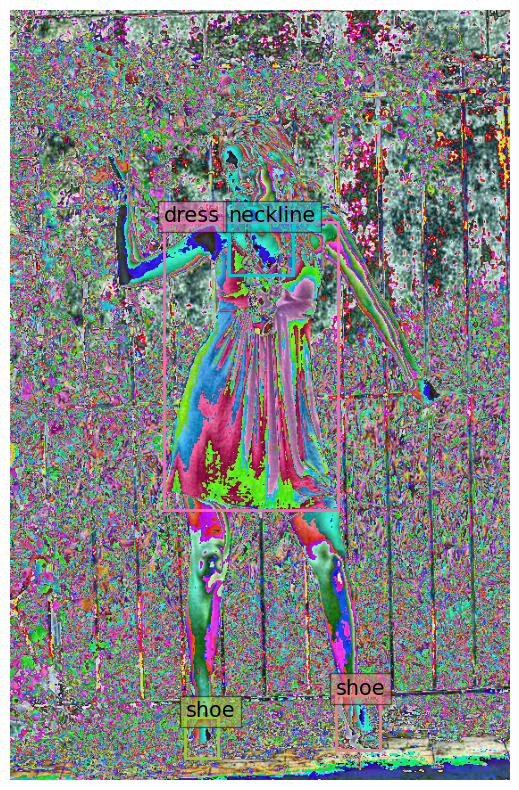
\includegraphics[width=0.45\textwidth]{images/yolos.png}
    \caption{Example of YOLOS feature extractor applied to an image}
\end{figure}

\textbf{Significance:} Directly feeding raw images into a model is inefficient and ineffective. Feature extractors preprocess images into consistent formats and value ranges, enabling deep learning models to focus on learning useful patterns instead of compensating for inconsistencies in raw input data.

\section{Fashion Product Images Dataset Cleaning}

The second dataset initially contained significant redundancies and irrelevant entries. Several preprocessing steps were undertaken:

\vspace{-1.25em}
\begin{enumerate}
    \setlength\itemsep{-1.05em}
    \item \textbf{Duplicate Removal:} Items with identical descriptions were removed to avoid training on repeated data.
    \item \textbf{Unknown Categories Exclusion:} Entries labeled as ``Unknown'' in the \texttt{product\_group\_name} were discarded to ensure all data belonged to meaningful, interpretable categories.
    \item \textbf{Token Length Filtering:} Since FashionCLIP has a token limit of 77, descriptions longer than 40 words were excluded to maintain safety margins and ensure compatibility.
    \item \textbf{Rare Product Types Removal:} Product types with very few samples (less than 10 occurrences) were eliminated to prevent skewed learning.
\end{enumerate}

After these steps, the original dataset of 1,05,542 products was reduced to 37,704 products. The remaining entries were then re-indexed to ensure a clean and continuous dataset.

Additionally, a random price was assigned to each item for downstream tasks, and the corresponding local image paths were constructed based on their article IDs.

\textbf{Significance:} These steps ensure that the final dataset is clean, consistent, and better suited for training vision-language models. Removing duplicates and rare categories avoids overfitting to irrelevant patterns, while maintaining concise descriptions ensures compatibility with the model's token limits.

After preprocessing, the dataset size was significantly reduced, resulting in a more manageable and high-quality subset ready for model training.
